\documentclass[10pt,letterpaper]{article}\usepackage[]{graphicx}\usepackage[]{color}
%% maxwidth is the original width if it is less than linewidth
%% otherwise use linewidth (to make sure the graphics do not exceed the margin)
\makeatletter
\def\maxwidth{ %
  \ifdim\Gin@nat@width>\linewidth
    \linewidth
  \else
    \Gin@nat@width
  \fi
}
\makeatother

\definecolor{fgcolor}{rgb}{0.345, 0.345, 0.345}
\newcommand{\hlnum}[1]{\textcolor[rgb]{0.686,0.059,0.569}{#1}}%
\newcommand{\hlstr}[1]{\textcolor[rgb]{0.192,0.494,0.8}{#1}}%
\newcommand{\hlcom}[1]{\textcolor[rgb]{0.678,0.584,0.686}{\textit{#1}}}%
\newcommand{\hlopt}[1]{\textcolor[rgb]{0,0,0}{#1}}%
\newcommand{\hlstd}[1]{\textcolor[rgb]{0.345,0.345,0.345}{#1}}%
\newcommand{\hlkwa}[1]{\textcolor[rgb]{0.161,0.373,0.58}{\textbf{#1}}}%
\newcommand{\hlkwb}[1]{\textcolor[rgb]{0.69,0.353,0.396}{#1}}%
\newcommand{\hlkwc}[1]{\textcolor[rgb]{0.333,0.667,0.333}{#1}}%
\newcommand{\hlkwd}[1]{\textcolor[rgb]{0.737,0.353,0.396}{\textbf{#1}}}%
\let\hlipl\hlkwb

\usepackage{framed}
\makeatletter
\newenvironment{kframe}{%
 \def\at@end@of@kframe{}%
 \ifinner\ifhmode%
  \def\at@end@of@kframe{\end{minipage}}%
  \begin{minipage}{\columnwidth}%
 \fi\fi%
 \def\FrameCommand##1{\hskip\@totalleftmargin \hskip-\fboxsep
 \colorbox{shadecolor}{##1}\hskip-\fboxsep
     % There is no \\@totalrightmargin, so:
     \hskip-\linewidth \hskip-\@totalleftmargin \hskip\columnwidth}%
 \MakeFramed {\advance\hsize-\width
   \@totalleftmargin\z@ \linewidth\hsize
   \@setminipage}}%
 {\par\unskip\endMakeFramed%
 \at@end@of@kframe}
\makeatother

\definecolor{shadecolor}{rgb}{.97, .97, .97}
\definecolor{messagecolor}{rgb}{0, 0, 0}
\definecolor{warningcolor}{rgb}{1, 0, 1}
\definecolor{errorcolor}{rgb}{1, 0, 0}
\newenvironment{knitrout}{}{} % an empty environment to be redefined in TeX

\usepackage{alltt}
\usepackage[top=0.85in,left=1.75in,footskip=0.75in]{geometry}

% amsmath and amssymb packages, useful for mathematical formulas and symbols
\usepackage{amsmath,amssymb}

% Use adjustwidth environment to exceed column width (see example table in text)
\usepackage{changepage}

% Use Unicode characters when possible
\usepackage[utf8x]{inputenc}

% textcomp package and marvosym package for additional characters
\usepackage{textcomp,marvosym}

% cite package, to clean up citations in the main text. Do not remove.
\usepackage{cite}

% Use nameref to cite supporting information files (see Supporting Information section for more info)
\usepackage{nameref,hyperref}

% line numbers
\usepackage[right]{lineno}

% ligatures disabled
\usepackage{microtype}
\DisableLigatures[f]{encoding = *, family = * }

% color can be used to apply background shading to table cells only
\usepackage[table]{xcolor}

% array package and thick rules for tables
\usepackage{array}

% adjust width of tikz tables or figures
\usepackage{adjustbox}

% bold math symbols package
\usepackage{bm}

% nice figures and captions
\usepackage{graphicx}

% diagrams or complicated equations
\usepackage{tikz}

% vertical and horizontal dashed lines
\usepackage{arydshln}

%\usepackage{floatflt}
%\usepackage{nonfloat}
\usepackage{float}
\usepackage{wrapfig}

%\renewcommand{\arraystretch}{1.2}
%\setlength{\tabcolsep}{12pt}

% create "+" rule type for thick vertical lines
\newcolumntype{+}{!{\vrule width 2pt}}

% create \thickcline for thick horizontal lines of variable length
\newlength\savedwidth
\newcommand\thickcline[1]{%
  \noalign{\global\savedwidth\arrayrulewidth\global\arrayrulewidth 2pt}%
  \cline{#1}%
  \noalign{\vskip\arrayrulewidth}%
  \noalign{\global\arrayrulewidth\savedwidth}%
}

% \thickhline command for thick horizontal lines that span the table
\newcommand\thickhline{\noalign{\global\savedwidth\arrayrulewidth\global\arrayrulewidth 2pt}%
\hline
\noalign{\global\arrayrulewidth\savedwidth}}


% Remove comment for double spacing
%\usepackage{setspace} 
%\doublespacing

% Text layout
% \raggedright
\setlength{\parindent}{0.5cm}
\textwidth 5.25in 
\textheight 8.75in

% Bold the 'Figure #' in the caption and separate it from the title/caption with a period
% Captions will be left justified
\usepackage[aboveskip=1pt,labelfont=bf,labelsep=period,justification=raggedright,singlelinecheck=off]{caption}
%\renewcommand{\figurename}{Supplementary Fig.}
\renewcommand{\thefigure}{S\arabic{figure}}

% Use the PLoS provided BiBTeX style
%\bibliographystyle{plos2015}


% Remove brackets from numbering in List of References
\makeatletter
\renewcommand{\@biblabel}[1]{\quad#1.}
\makeatother

% define theorem and definition environments commands
\newtheorem{theorem}{Theorem}[section]
\newtheorem{definition}{Definition}[section]

% Header and Footer with logo
\usepackage{lastpage,fancyhdr,graphicx}
\usepackage{epstopdf}
%\pagestyle{myheadings}
\pagestyle{fancy}
\fancyhf{}
%\setlength{\headheight}{27.023pt}
%\lhead{\includegraphics[width=2.0in]{PLOS-submission.eps}}
\rfoot{\thepage/\pageref{LastPage}}
\renewcommand{\headrulewidth}{0pt}
\renewcommand{\footrule}{\hrule height 2pt \vspace{2mm}}
\fancyheadoffset[L]{2.25in}
% \fancyfootoffset[L]{1.25in}
\lfoot{\today}


\restylefloat{figure}


%% Include all macros below

\newcommand{\lorem}{{\bf LOREM}}
\newcommand{\ipsum}{{\bf IPSUM}}

\def\lf{\left\lfloor}   
\def\rf{\right\rfloor}

\def\ri{R_i}
\def\rj{R_j}
\def\kmi{k_{M_i}}
\def\khi{k_{H_i}}
\def\hji{H_{j_i}}
\def\ma{\overline{M}_a}
\def\ha{\overline{H}_a}
\def\mnu{M_\nu}
\def\hnu{H_\nu}
\def\myd{\text{diff}}
\def\ka{\bar{k}_\alpha}
\def\mji{M_{j_i}}

%% END MACROS SECTION
\IfFileExists{upquote.sty}{\usepackage{upquote}}{}
\begin{document}
\vspace*{0.2in}

% Title must be 250 characters or less.
% \begin{flushleft}
{\Large	
	\textbf\newline{Supplementary figures} % Please use "sentence case" for title and headings (capitalize only the first word in a title (or heading), the first word in a subtitle (or subheading), and any proper nouns).	
}

\begin{figure}[H]
	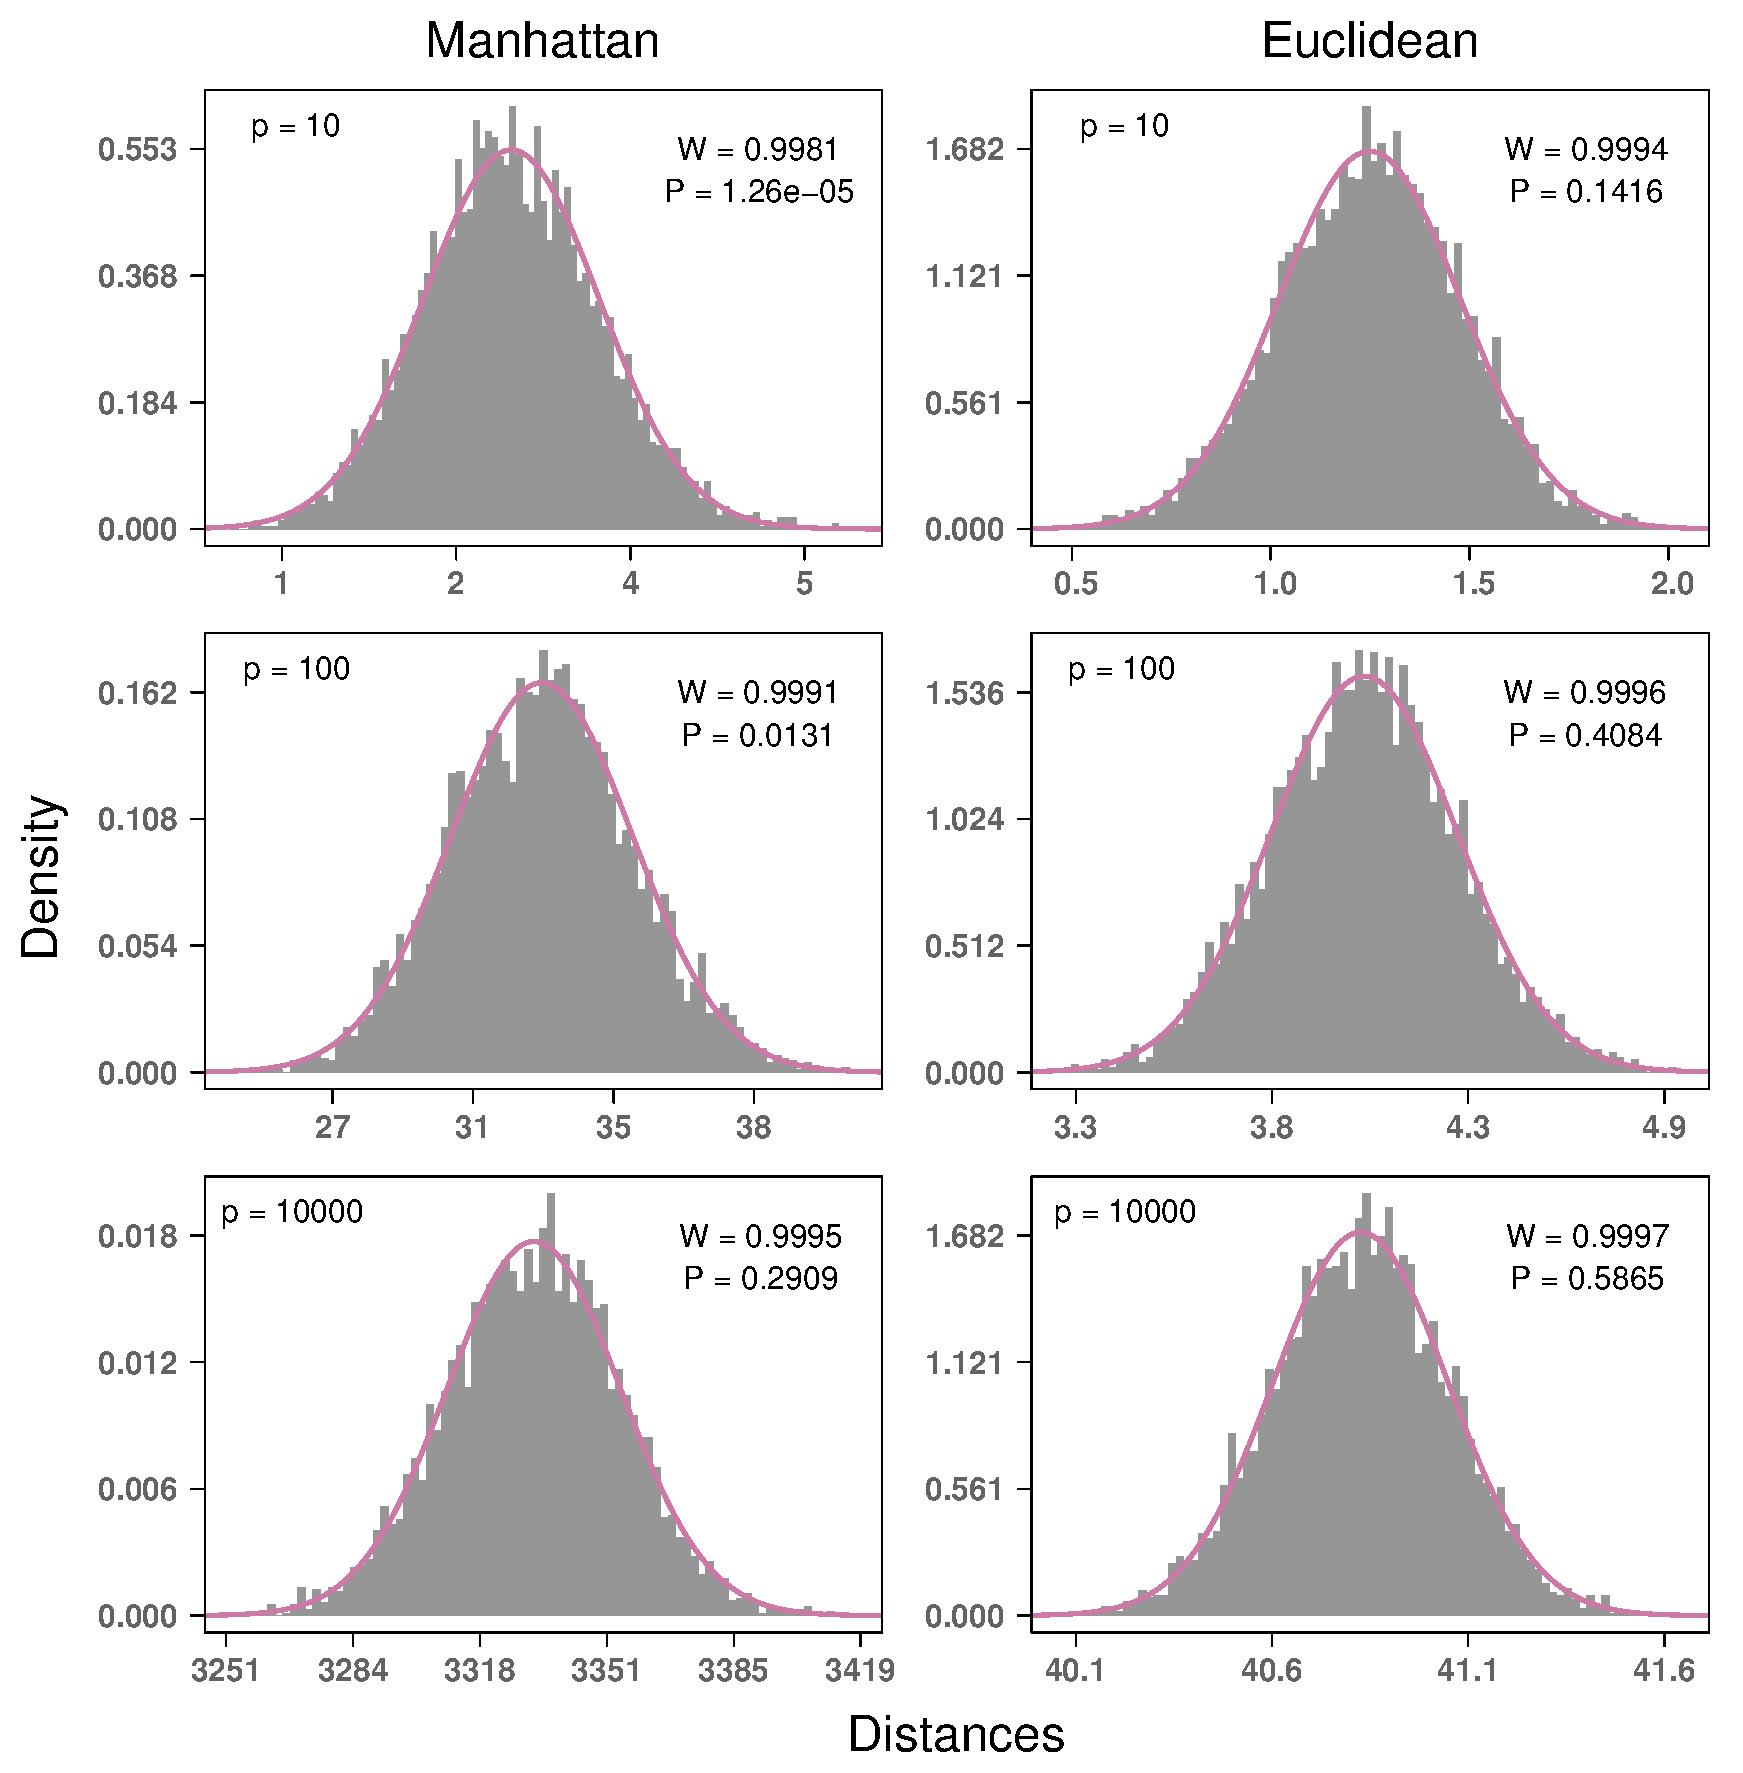
\includegraphics[width=\textwidth]{central_limit_hist_uniform_standard.pdf}
	\caption{This will be a caption. This will be a caption. This will be a caption. This will be a caption. This will be a caption. This will be a caption. This will be a caption. This will be a caption. This will be a caption. This will be a caption. This will be a caption. This will be a caption. This will be a caption. This will be a caption. This will be a caption. This will be a caption. This will be a caption. This will be a caption. This will be a caption. This will be a caption. This will be a caption. This will be a caption. This will be a caption. This will be a caption. This will be a caption. This will be a caption. This will be a caption. This will be a caption. This will be a caption. This will be a caption. This will be a caption. This will be a caption. This will be a caption. This will be a caption. This will be a caption. This will be a caption. This will be a caption. This will be a caption.}
\end{figure}

\begin{figure}[H]
	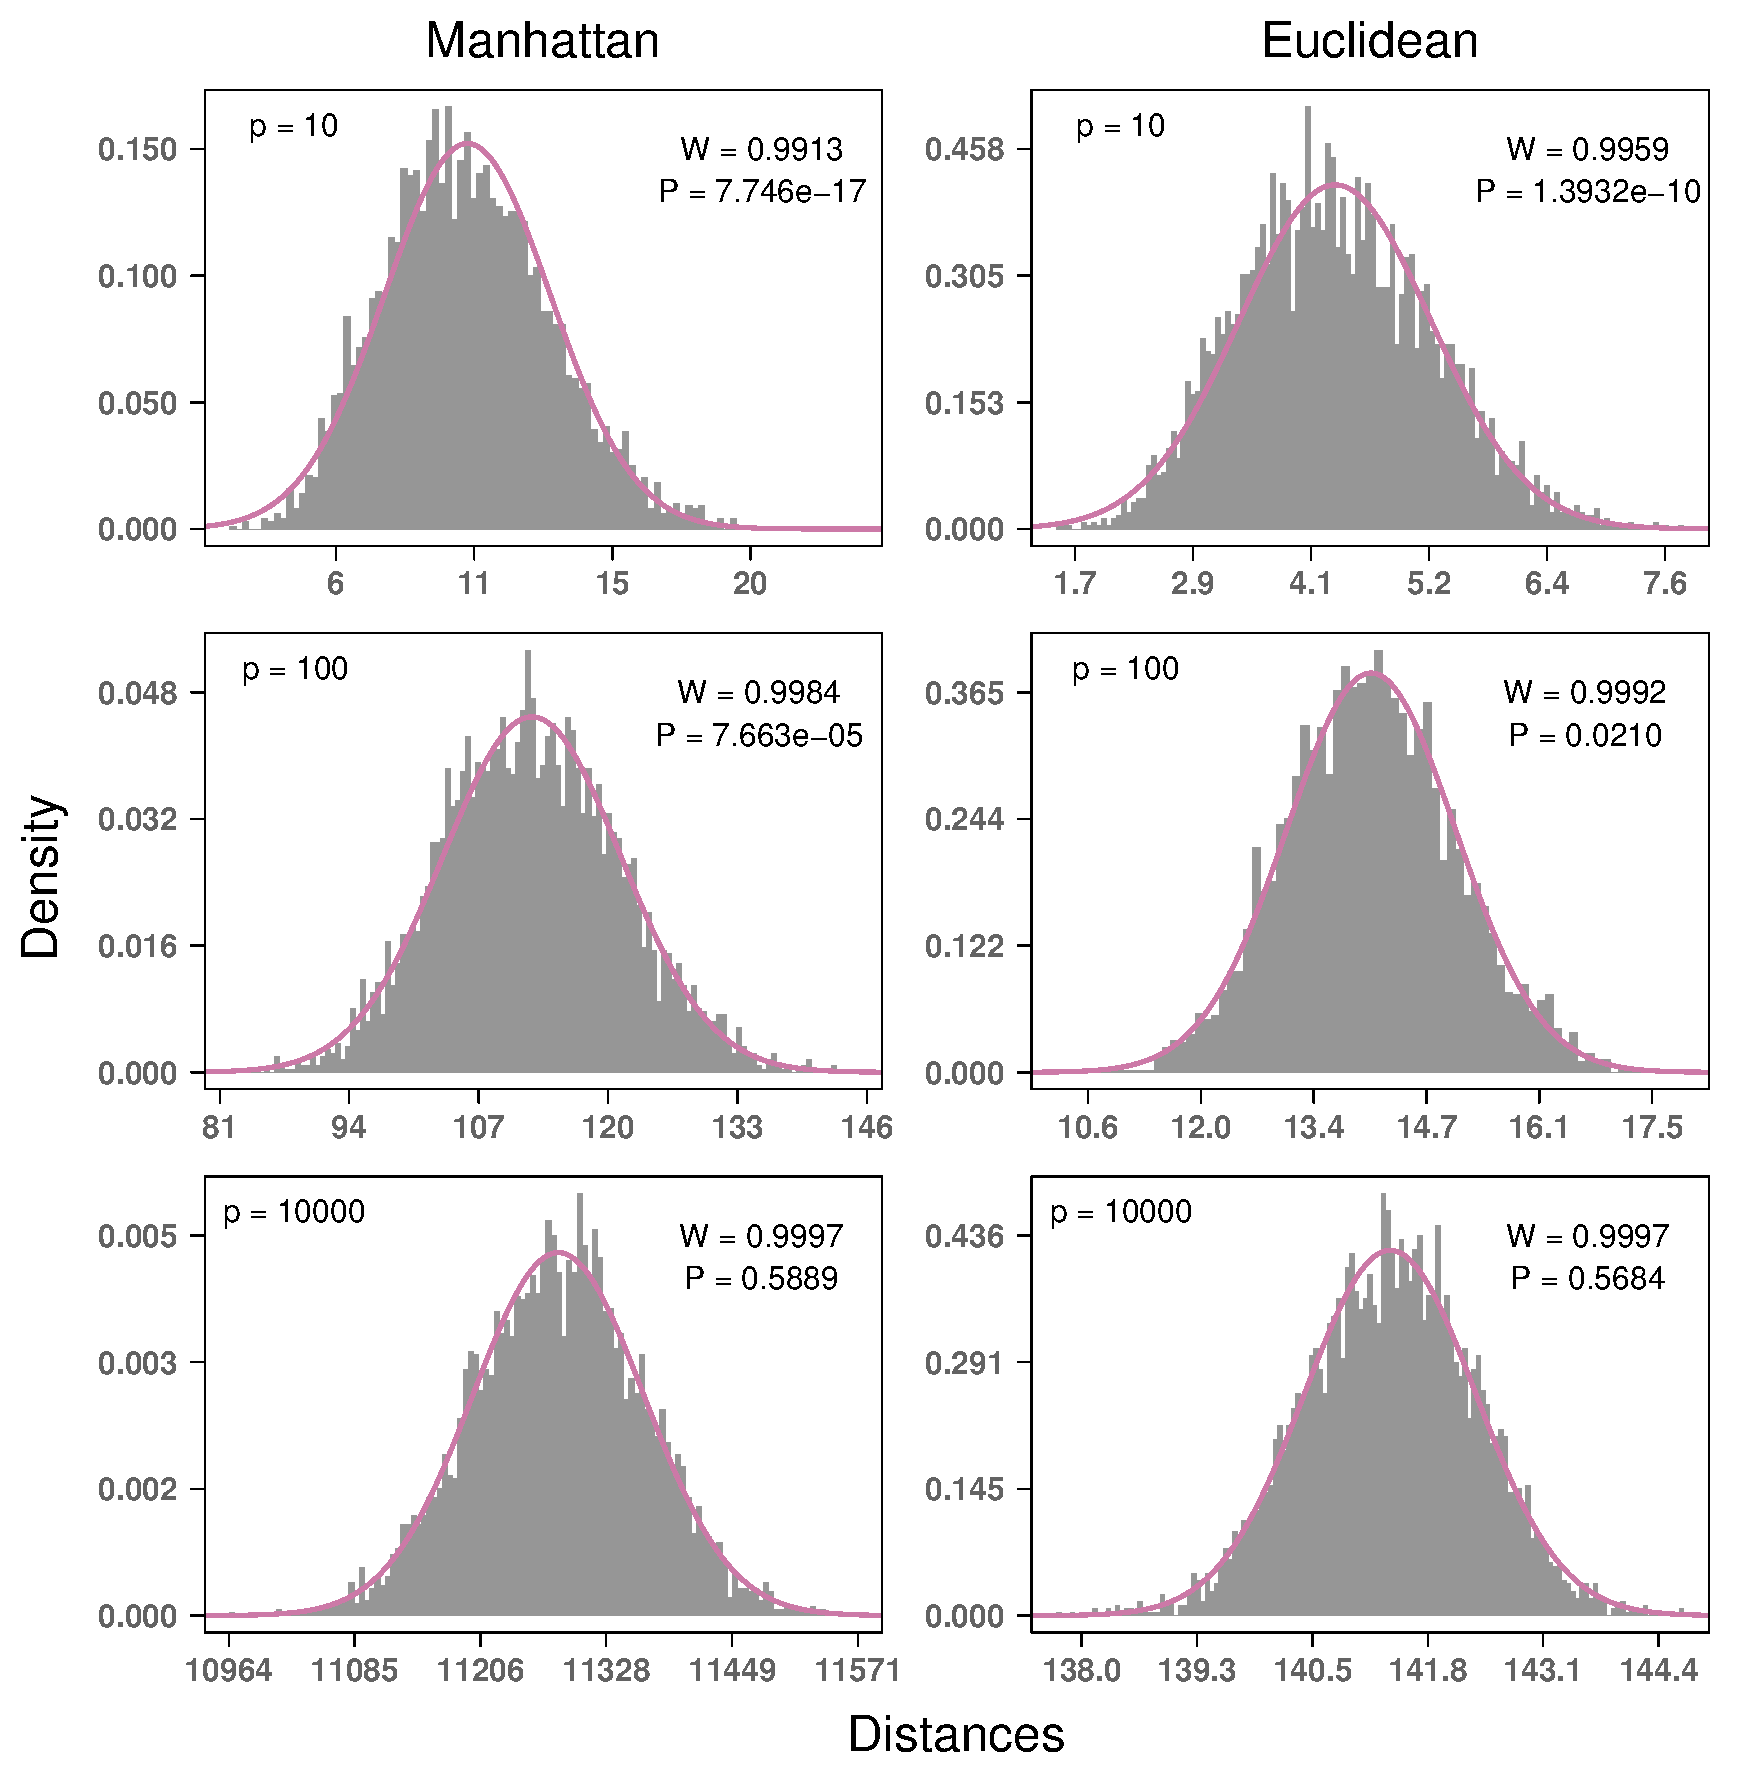
\includegraphics[width=\textwidth]{central_limit_hist_normal_standard.pdf}
	\caption{This will be a caption. This will be a caption. This will be a caption. This will be a caption. This will be a caption. This will be a caption. This will be a caption. This will be a caption. This will be a caption. This will be a caption. This will be a caption. This will be a caption. This will be a caption. This will be a caption. This will be a caption. This will be a caption. This will be a caption. This will be a caption. This will be a caption. This will be a caption. This will be a caption. This will be a caption. This will be a caption. This will be a caption. This will be a caption. This will be a caption. This will be a caption. This will be a caption. This will be a caption. This will be a caption. This will be a caption. This will be a caption. This will be a caption. This will be a caption. This will be a caption. This will be a caption. This will be a caption. This will be a caption.}
\end{figure}

\begin{figure}[H]
	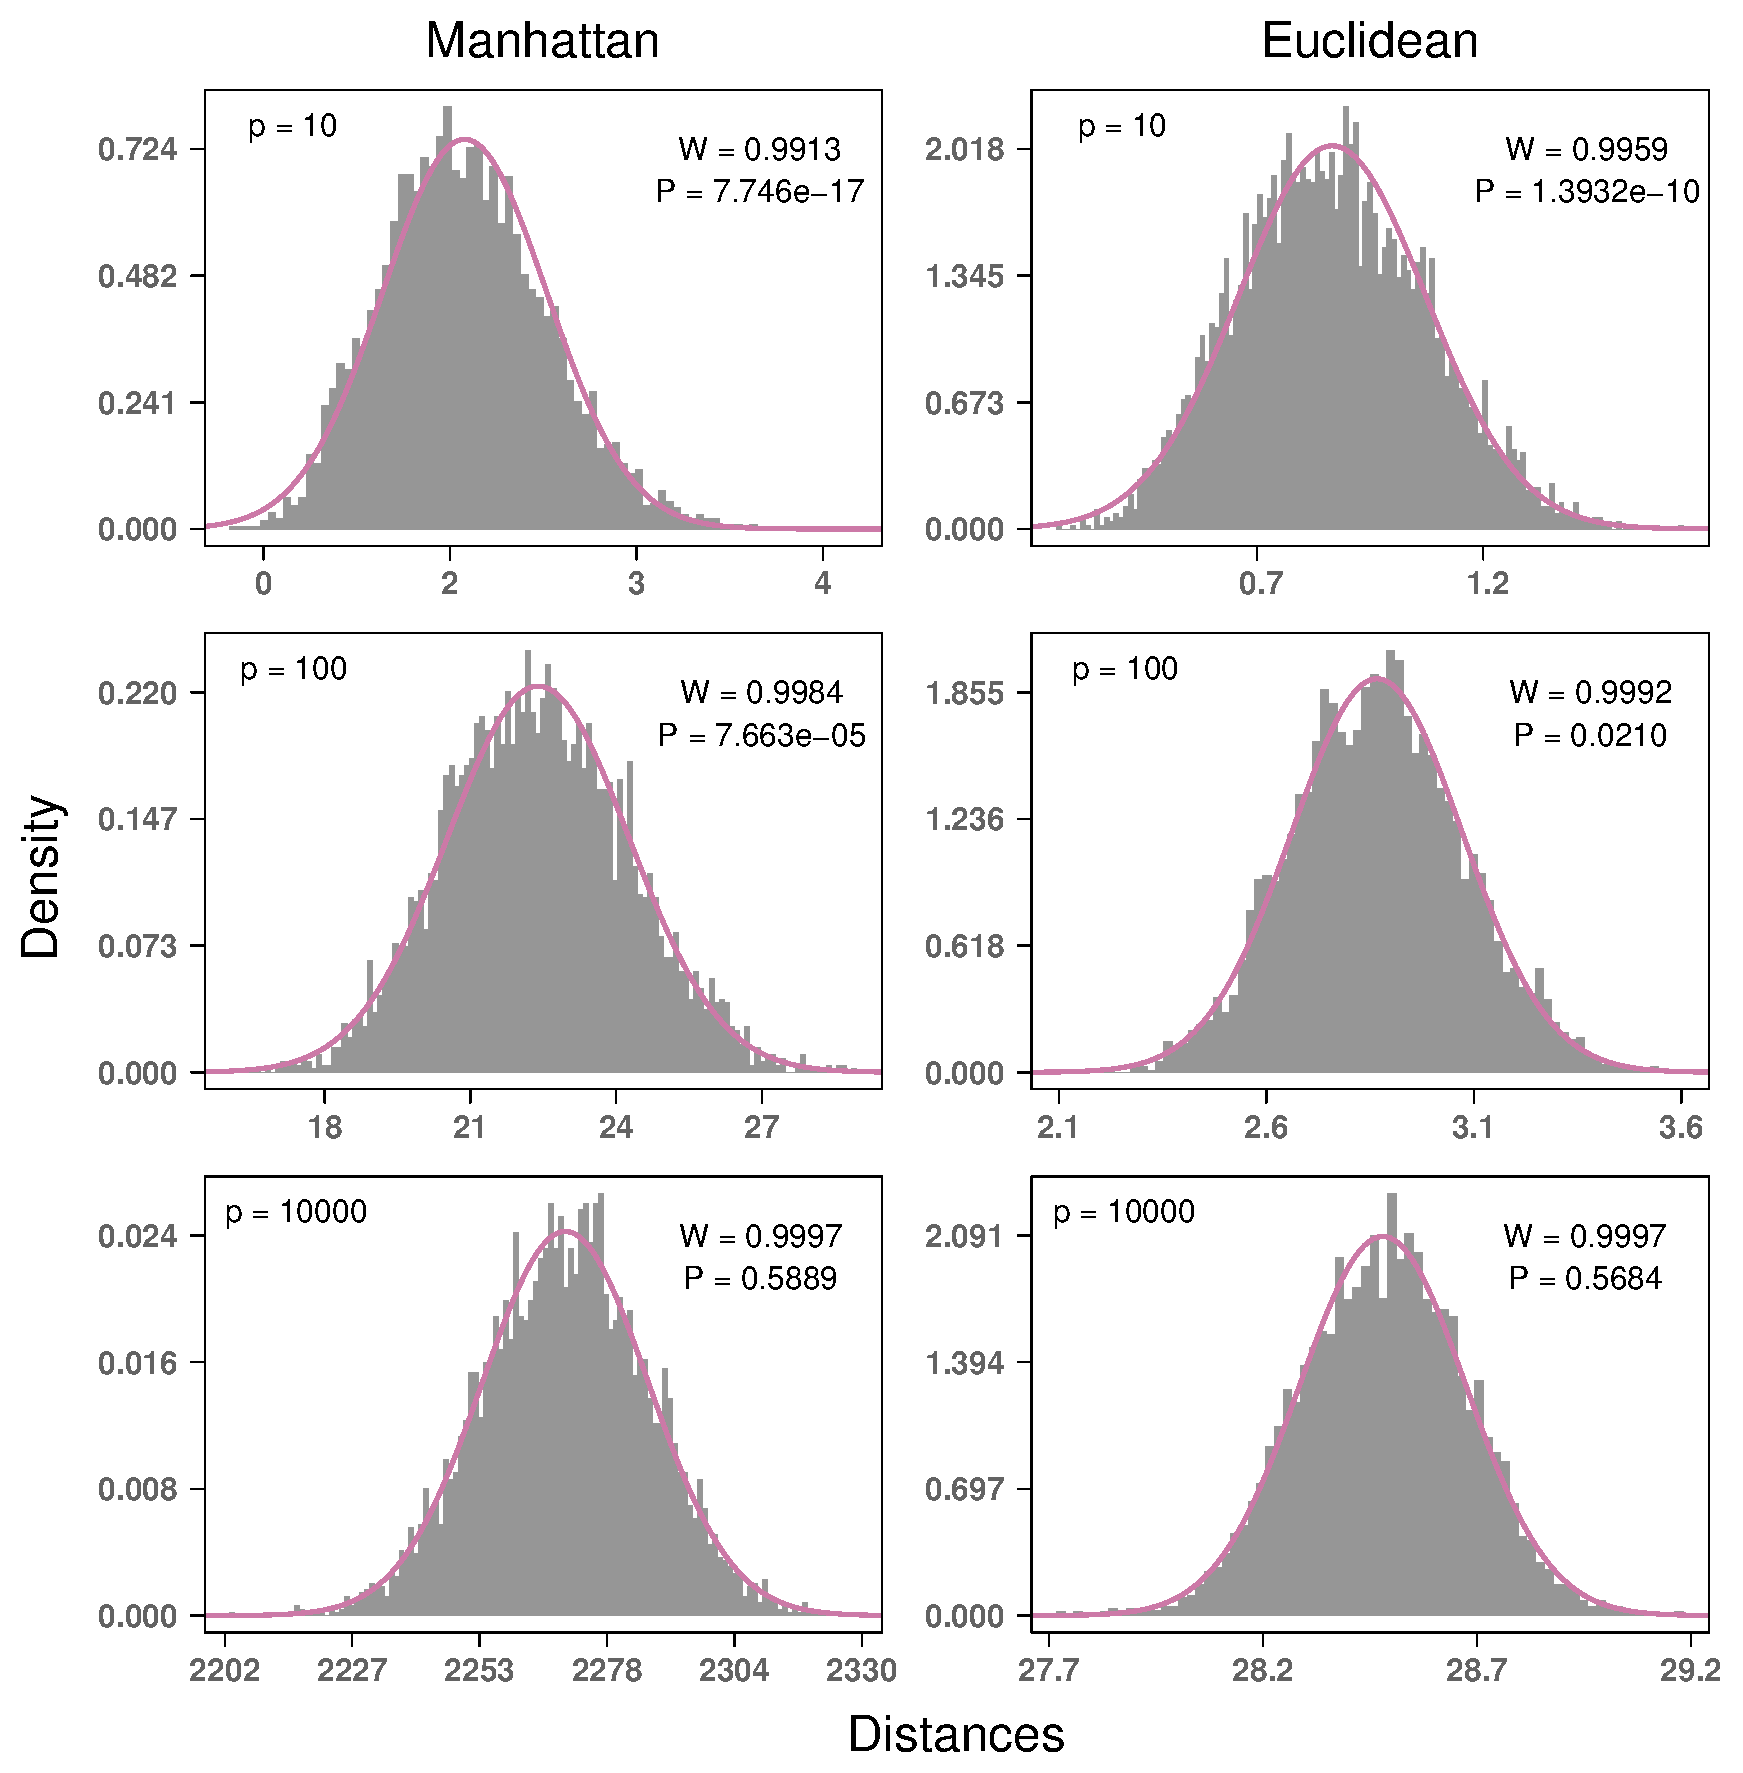
\includegraphics[width=\textwidth]{central_limit_hist_normal_max-min.pdf}
	\caption{This will be a caption. This will be a caption. This will be a caption. This will be a caption. This will be a caption. This will be a caption. This will be a caption. This will be a caption. This will be a caption. This will be a caption. This will be a caption. This will be a caption. This will be a caption. This will be a caption. This will be a caption. This will be a caption. This will be a caption. This will be a caption. This will be a caption. This will be a caption. This will be a caption. This will be a caption. This will be a caption. This will be a caption. This will be a caption. This will be a caption. This will be a caption. This will be a caption. This will be a caption. This will be a caption. This will be a caption. This will be a caption. This will be a caption. This will be a caption. This will be a caption. This will be a caption. This will be a caption. This will be a caption.}
\end{figure}

\begin{figure}[H]
	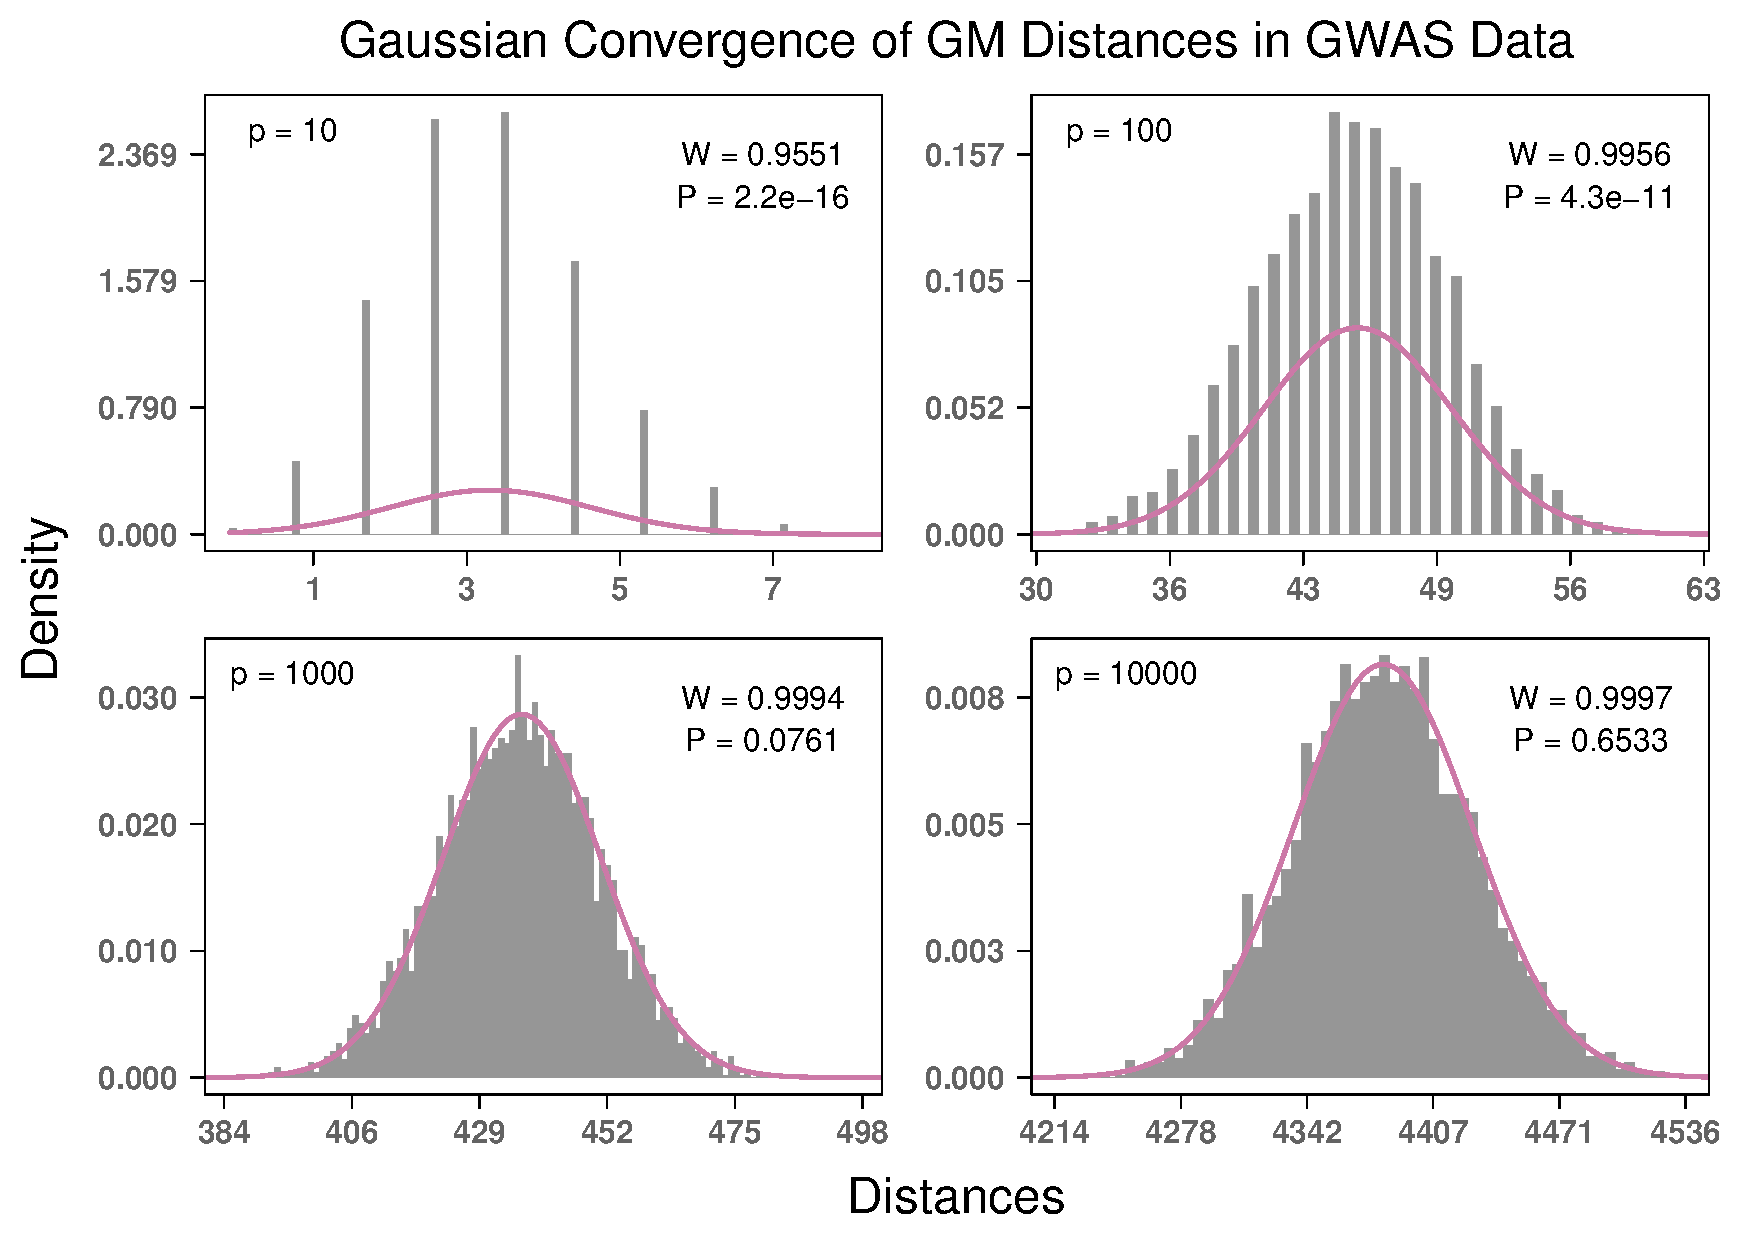
\includegraphics[width=\textwidth]{central_limit_hist_gwas_GM.pdf}
	\caption{This will be a caption. This will be a caption. This will be a caption. This will be a caption. This will be a caption. This will be a caption. This will be a caption. This will be a caption. This will be a caption. This will be a caption. This will be a caption. This will be a caption. This will be a caption. This will be a caption. This will be a caption. This will be a caption. This will be a caption. This will be a caption. This will be a caption. This will be a caption. This will be a caption. This will be a caption. This will be a caption. This will be a caption. This will be a caption. This will be a caption. This will be a caption. This will be a caption. This will be a caption. This will be a caption. This will be a caption. This will be a caption. This will be a caption. This will be a caption. This will be a caption. This will be a caption. This will be a caption. This will be a caption.}
\end{figure}

\begin{figure}[H]
	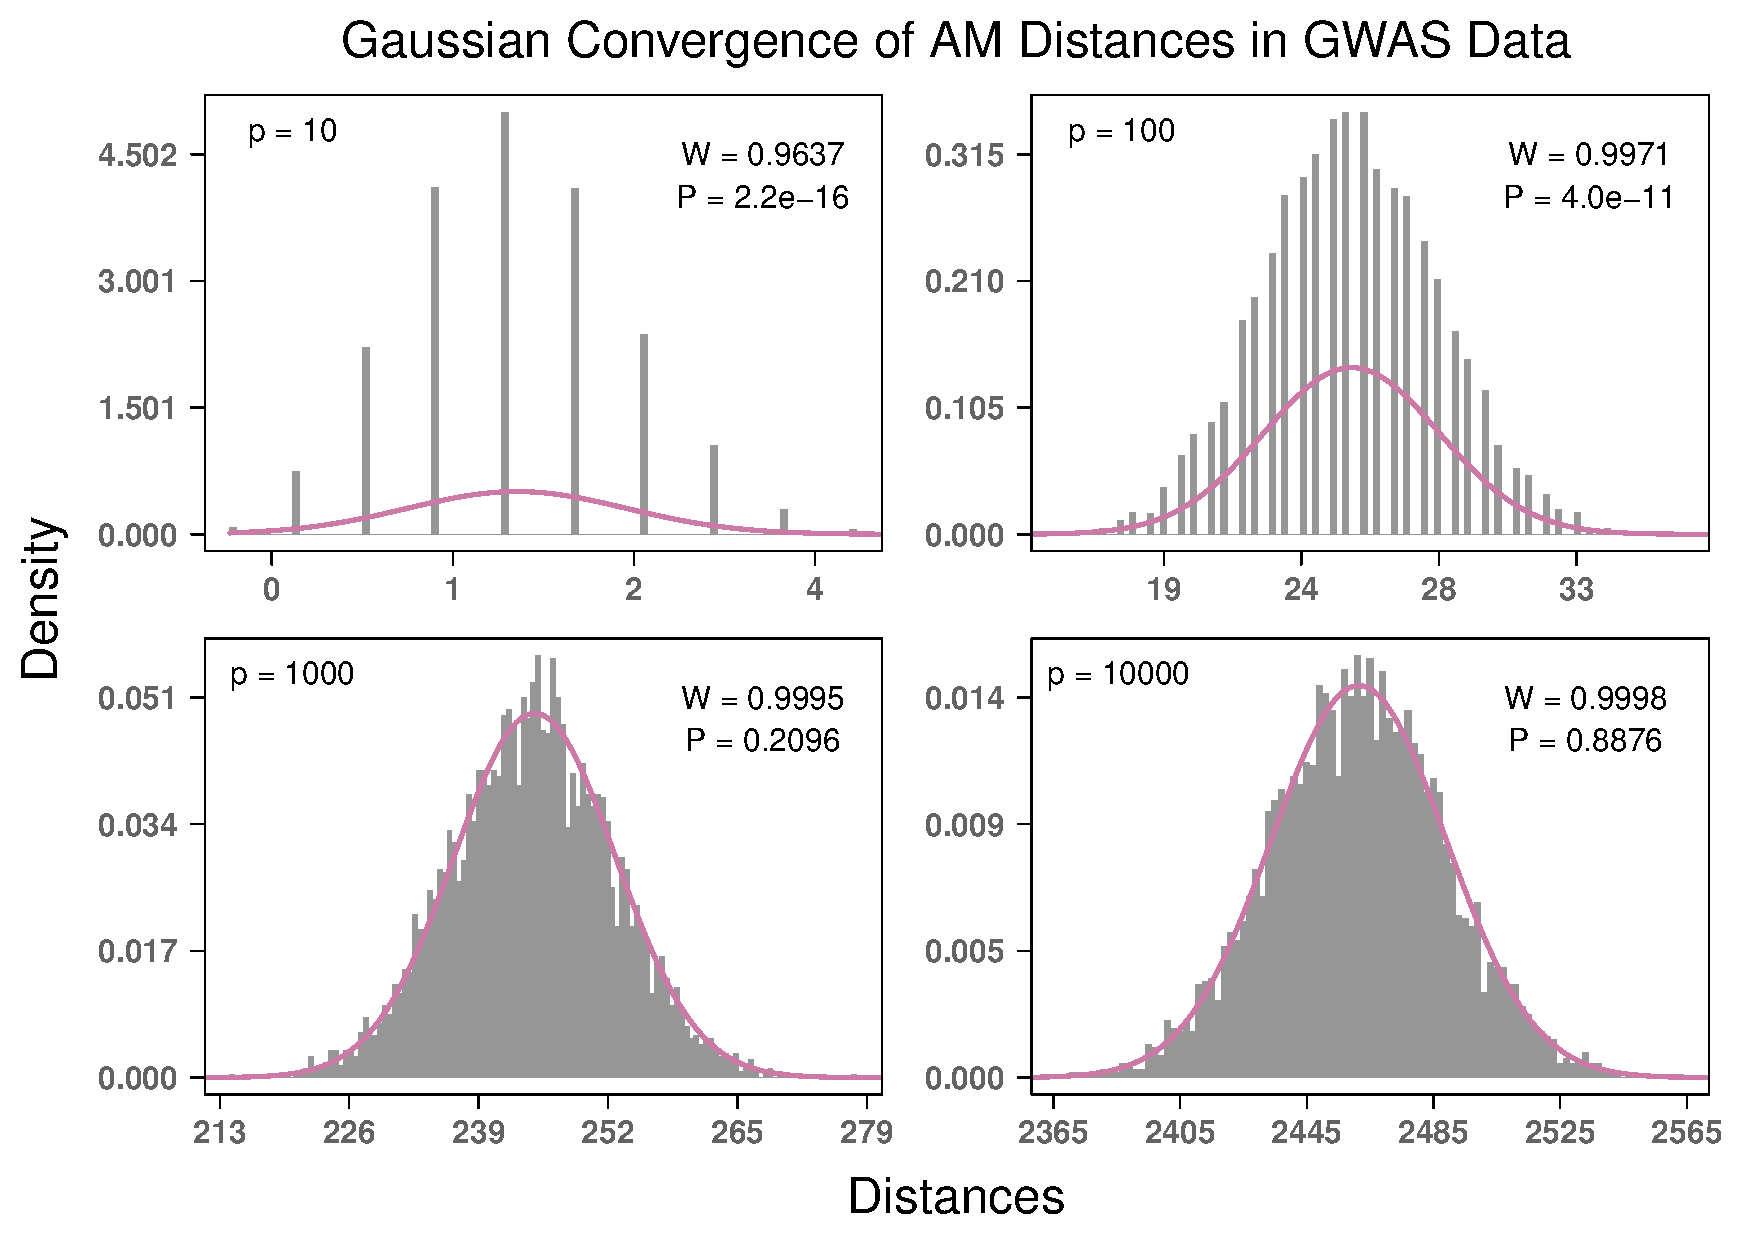
\includegraphics[width=\textwidth]{central_limit_hist_gwas_AM.pdf}
	\caption{This will be a caption. This will be a caption. This will be a caption. This will be a caption. This will be a caption. This will be a caption. This will be a caption. This will be a caption. This will be a caption. This will be a caption. This will be a caption. This will be a caption. This will be a caption. This will be a caption. This will be a caption. This will be a caption. This will be a caption. This will be a caption. This will be a caption. This will be a caption. This will be a caption. This will be a caption. This will be a caption. This will be a caption. This will be a caption. This will be a caption. This will be a caption. This will be a caption. This will be a caption. This will be a caption. This will be a caption. This will be a caption. This will be a caption. This will be a caption. This will be a caption. This will be a caption. This will be a caption. This will be a caption.}
\end{figure}

\begin{figure}[H]
	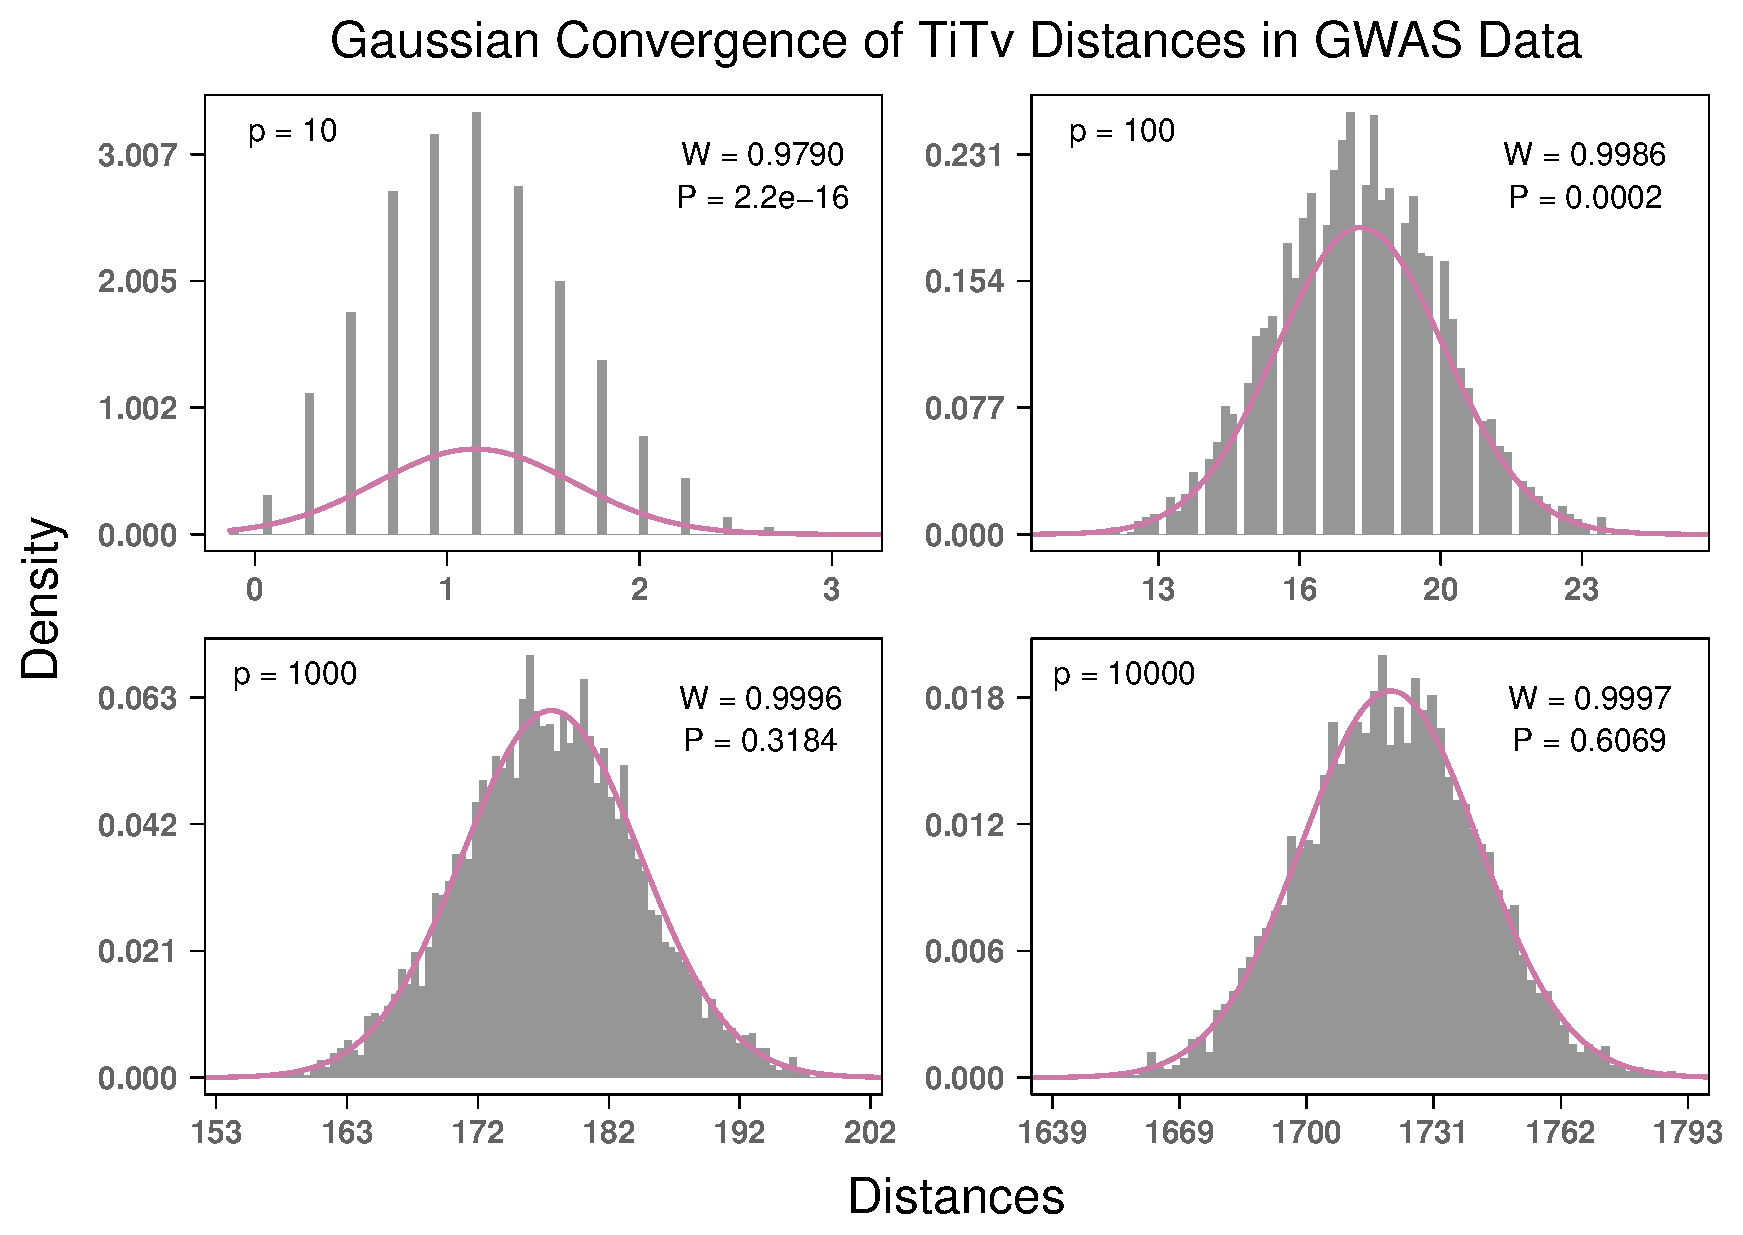
\includegraphics[width=\textwidth]{central_limit_hist_gwas_TiTv.pdf}
	\caption{This will be a caption. This will be a caption. This will be a caption. This will be a caption. This will be a caption. This will be a caption. This will be a caption. This will be a caption. This will be a caption. This will be a caption. This will be a caption. This will be a caption. This will be a caption. This will be a caption. This will be a caption. This will be a caption. This will be a caption. This will be a caption. This will be a caption. This will be a caption. This will be a caption. This will be a caption. This will be a caption. This will be a caption. This will be a caption. This will be a caption. This will be a caption. This will be a caption. This will be a caption. This will be a caption. This will be a caption. This will be a caption. This will be a caption. This will be a caption. This will be a caption. This will be a caption. This will be a caption. This will be a caption.}
\end{figure}

\begin{figure}[H]
	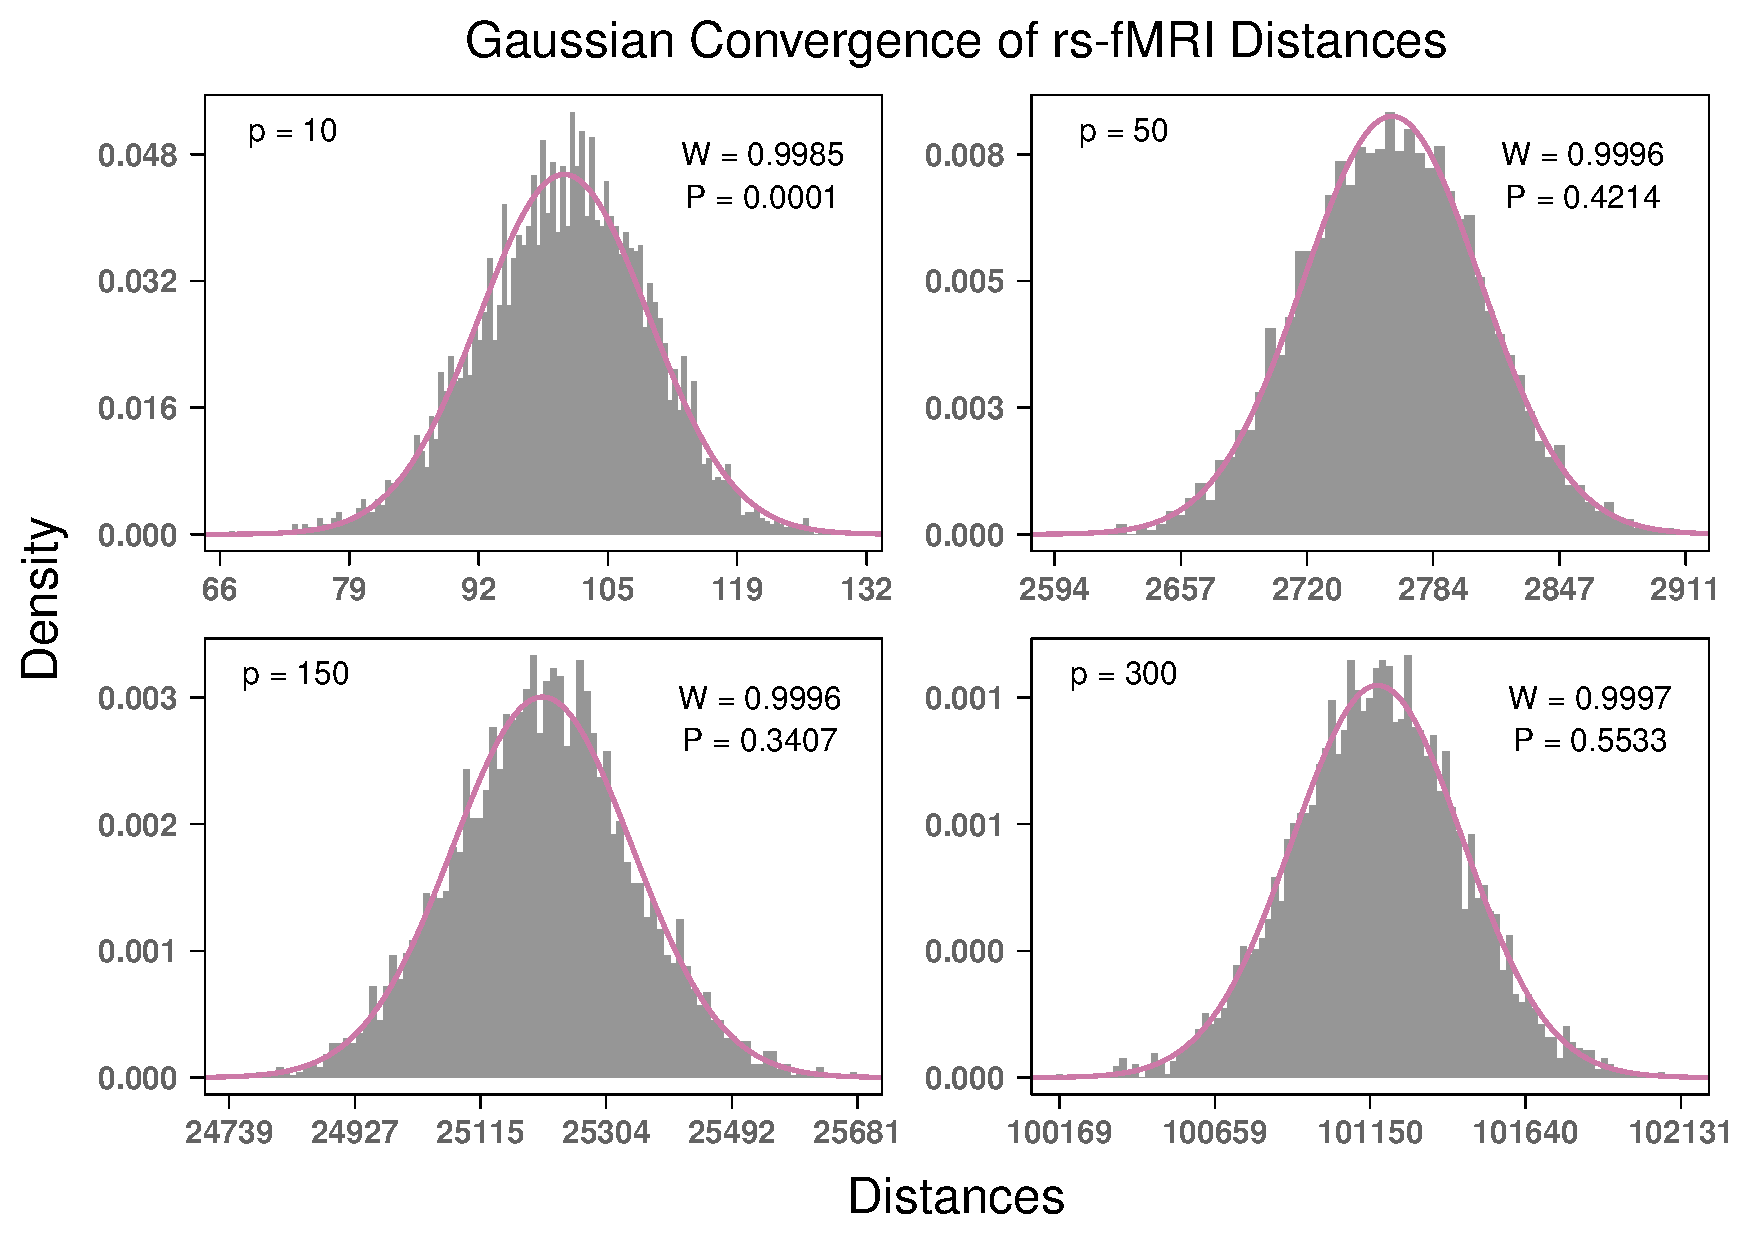
\includegraphics[width=\textwidth]{central_limit_hist_rs-fMRI_standard.pdf}
	\caption{This will be a caption. This will be a caption. This will be a caption. This will be a caption. This will be a caption. This will be a caption. This will be a caption. This will be a caption. This will be a caption. This will be a caption. This will be a caption. This will be a caption. This will be a caption. This will be a caption. This will be a caption. This will be a caption. This will be a caption. This will be a caption. This will be a caption. This will be a caption. This will be a caption. This will be a caption. This will be a caption. This will be a caption. This will be a caption. This will be a caption. This will be a caption. This will be a caption. This will be a caption. This will be a caption. This will be a caption. This will be a caption. This will be a caption. This will be a caption. This will be a caption. This will be a caption. This will be a caption. This will be a caption.}
\end{figure}

\begin{figure}[H]
	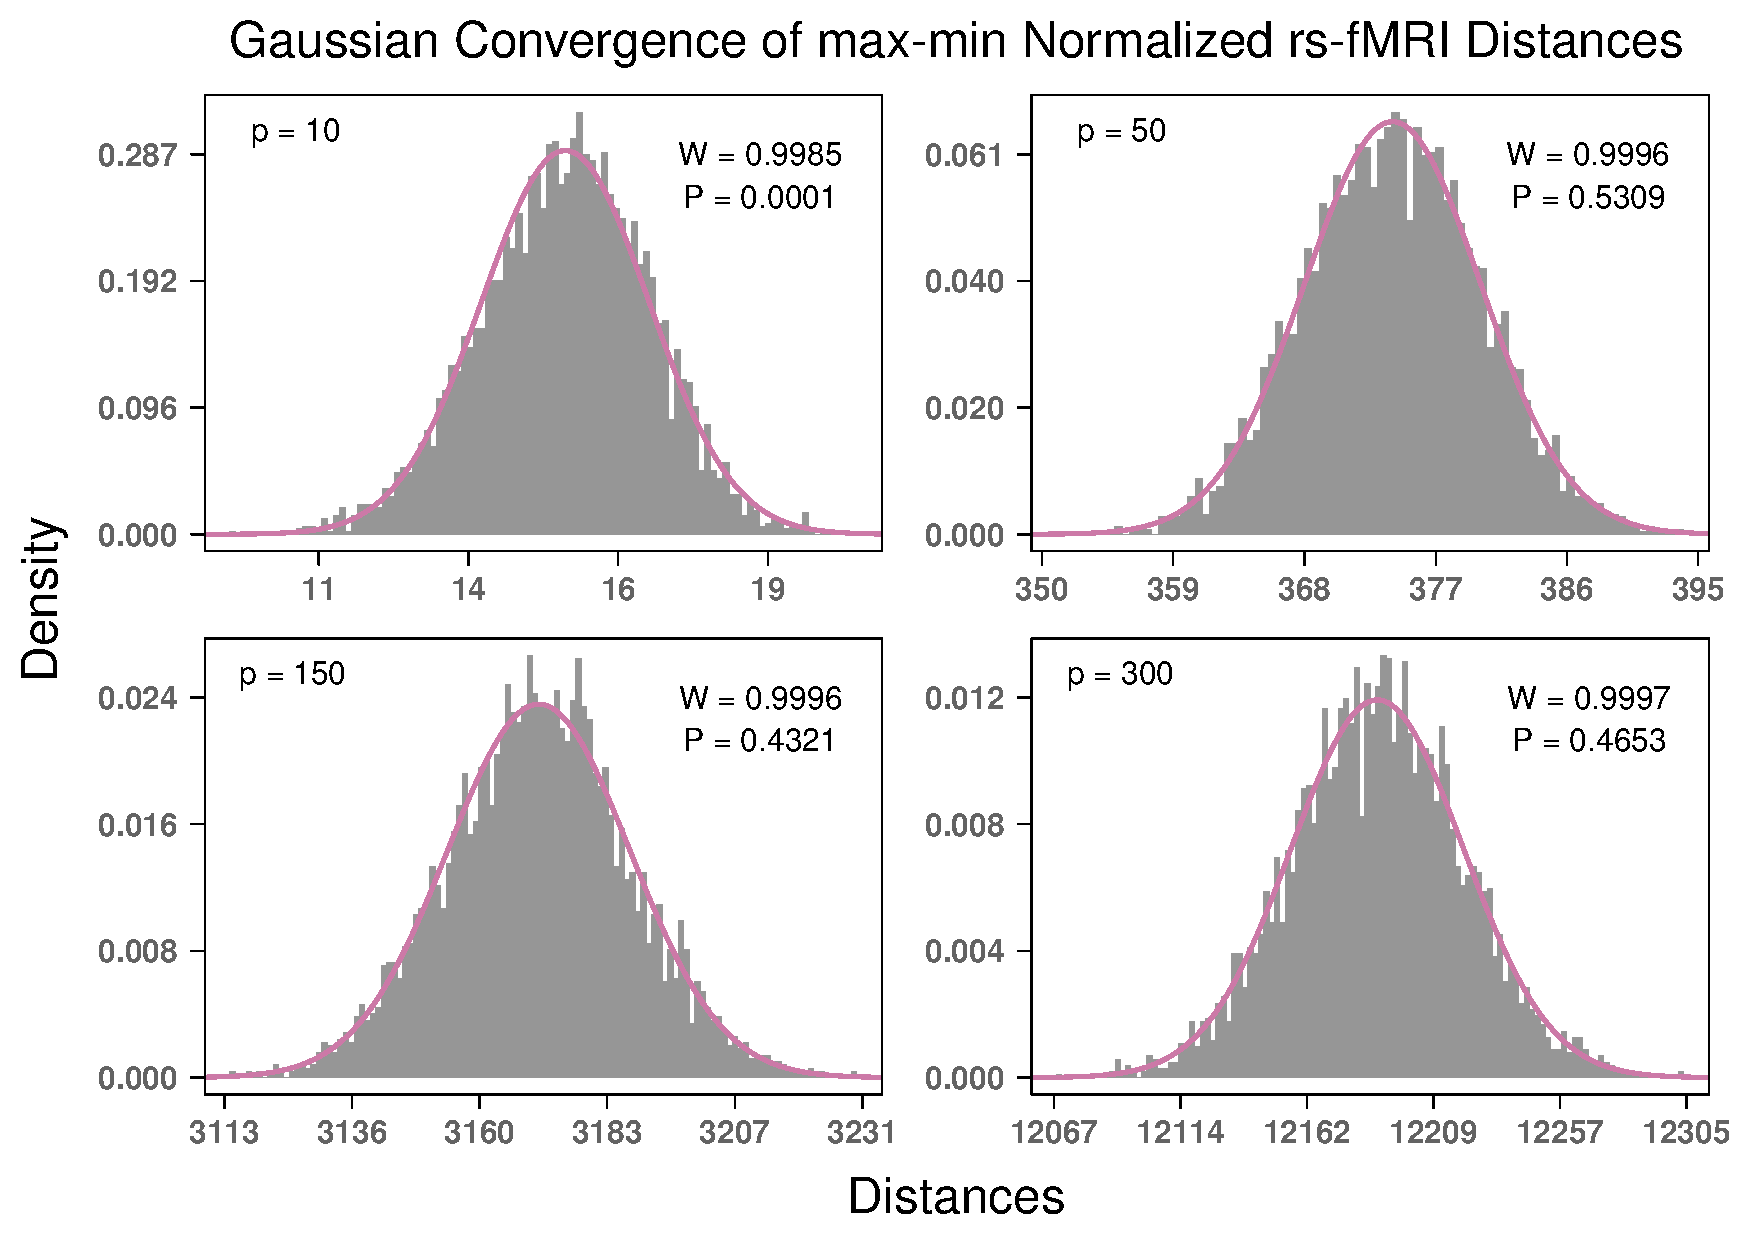
\includegraphics[width=\textwidth]{central_limit_hist_rs-fMRI_max-min.pdf}
	\caption{This will be a caption. This will be a caption. This will be a caption. This will be a caption. This will be a caption. This will be a caption. This will be a caption. This will be a caption. This will be a caption. This will be a caption. This will be a caption. This will be a caption. This will be a caption. This will be a caption. This will be a caption. This will be a caption. This will be a caption. This will be a caption. This will be a caption. This will be a caption. This will be a caption. This will be a caption. This will be a caption. This will be a caption. This will be a caption. This will be a caption. This will be a caption. This will be a caption. This will be a caption. This will be a caption. This will be a caption. This will be a caption. This will be a caption. This will be a caption. This will be a caption. This will be a caption. This will be a caption. This will be a caption.}
\end{figure}

%\bibliographystyle{unsrt}
%\bibliography{BoD}   % name of bib file
\end{document}
